\documentclass{standalone}
\usepackage{tikz}
\usepackage{amssymb}
\usetikzlibrary{decorations.markings}

\begin{document}

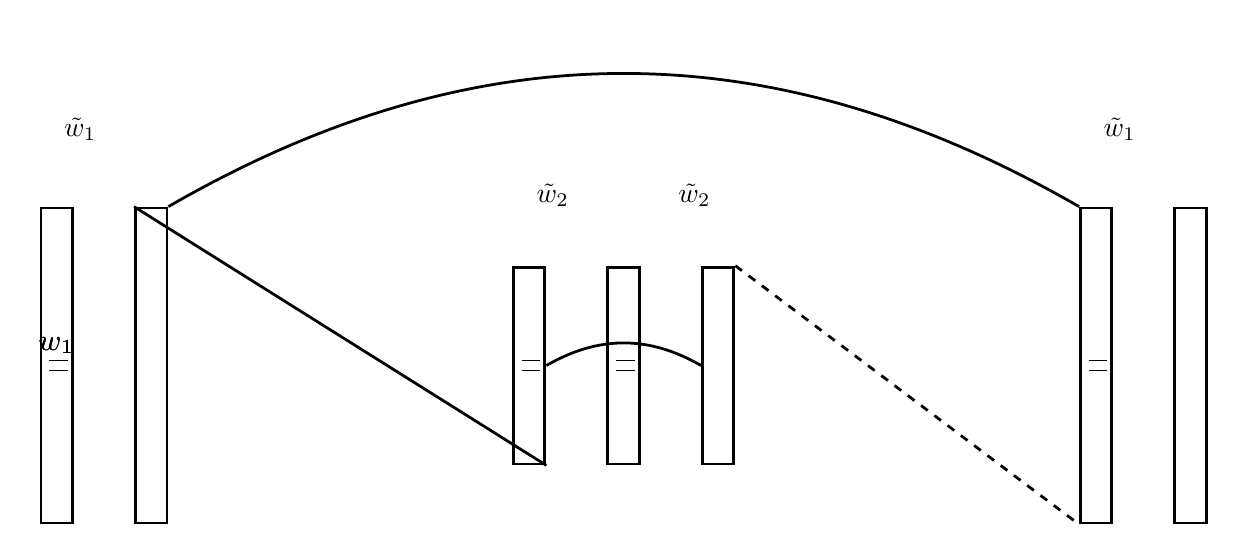
\begin{tikzpicture}[scale=1.2]

  % Define styles for easier use
  \tikzset{
    bar/.style={draw, line width=1pt, minimum width=0.4cm, minimum height=#1},
    edge label/.style={font=\small, midway, auto}
  }

  % Draw vertical bars (left group)
  \node[bar=4cm] (L1) at (0,0) {};
  \node[bar=4cm] (L2) at (1,0) {};

  % Draw horizontal lines within left group
  \draw (L1.west) ++(0.1,-0.05) -- ++(0.2,0); % Bottom line
  \draw (L1.west) ++(0.1,0.05) -- ++(0.2,0);  % Top line
  \node at (0.25,2.5) {$\tilde{w}_1$};

  % Draw vertical bars (middle group)
  \node[bar=2.5cm] (M1) at (5,0) {};
  \node[bar=2.5cm] (M2) at (6,0) {};
  \node[bar=2.5cm] (M3) at (7,0) {};

  % Draw horizontal lines within middle group
  \draw (M1.west) ++(0.1,-0.05) -- ++(0.2,0); % Bottom line
  \draw (M1.west) ++(0.1,0.05) -- ++(0.2,0);  % Top line
  \node at (5.25,1.8) {$\tilde{w}_2$};

  \draw (M2.west) ++(0.1,-0.05) -- ++(0.2,0); % Bottom line
  \draw (M2.west) ++(0.1,0.05) -- ++(0.2,0);  % Top line
  \node at (6.75,1.8) {$\tilde{w}_2$};

  % Draw vertical bars (right group)
  \node[bar=4cm] (R1) at (11,0) {};
  \node[bar=4cm] (R2) at (12,0) {};

  % Draw horizontal lines within right group
  \draw (R1.west) ++(0.1,-0.05) -- ++(0.2,0); % Bottom line
  \draw (R1.west) ++(0.1,0.05) -- ++(0.2,0);  % Top line
  \node at (11.25,2.5) {$\tilde{w}_1$};

  % Draw arcs and connecting lines
  % Top arc connecting left and right groups
  \draw[line width=1pt] (L2.north east) to[out=30,in=150] (R1.north west);

  % Middle arc connecting bars in middle group
  \draw[line width=1pt] (M1.east) to[out=30,in=150] (M3.west);

  % Diagonal lines
  \draw[line width=1pt] (L2.north west) -- (M1.south east);
  \node[edge label] at (2.5,2.5) {$w_1$};

  \draw[line width=1pt, dashed] (M3.north east) -- (R1.south west);
  \node[edge label] at (9.5,2.5) {$w_1$};

\end{tikzpicture}

\end{document}